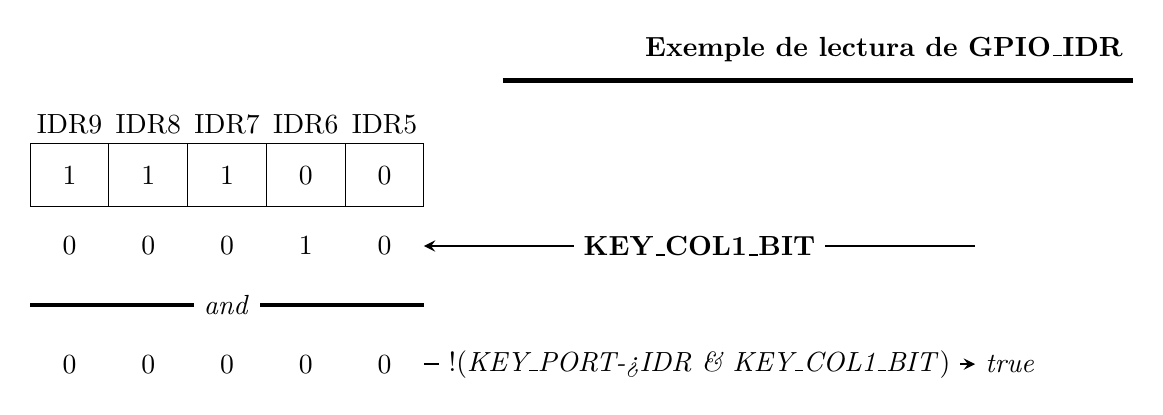
\begin{tikzpicture}
    \draw[ultra thick] (6, 1.6) -- (14, 1.6);
    \node[left] at(14, 2) {\textbf{Exemple de lectura de GPIO\_IDR}};

    \foreach \i in {5,...,9}
    {\node[above] at (2.5 - \i + 7, 0.8) {IDR\i};}
    \foreach \i in {0,...,4}
    {\draw[] (\i, 0) rectangle ++(1, 0.8);}

    \node[] at (0.5, 0.4) {1};
    \node[] at (1.5, 0.4) {1};
    \node[] at (2.5, 0.4) {1};
    \node[] at (3.5, 0.4) {0};
    \node[] at (4.5, 0.4) {0};

    \draw[thick, -stealth] (12, -0.5) -- (5, -0.5);
    \node[fill = white] at (8.5, -0.5){\textbf{KEY\_COL1\_BIT}};

    \node[] at (0.5, -0.5) {0};
    \node[] at (1.5, -0.5) {0};
    \node[] at (2.5, -0.5) {0};
    \node[] at (3.5, -0.5) {1};
    \node[] at (4.5, -0.5) {0};

    \draw[ultra thick] (0, -1.25) -- ++ (5, 0);
    \node[fill=white] at(2.5, -1.25){\textit{and}};

    \node[] at (0.5, -2) {0};
    \node[] at (1.5, -2) {0};
    \node[] at (2.5, -2) {0};
    \node[] at (3.5, -2) {0};
    \node[] at (4.5, -2) {0};

    \draw[thick, -stealth] (5, -2) -- (12, -2)node[right] {\textit{true}};
    \node[fill = white] at (8.5, -2){!(\textit{KEY\_PORT->IDR \& KEY\_COL1\_BIT})};
\end{tikzpicture}